\documentclass[
  manuscript=article,
  layout=preprint,
  year=2026,
  volume=x,
]{extra/joas}

\doi{xx.xxxxx/joas.xxxx.xxxx}

\received {}
\revised  {}
\accepted {}
\published{}

\editor{}

\reviewers{}

\addbibresource{reference.bib}

\title{Post-Operational Taxi-Out Time Estimation from Open Ground Tracks and Flight Records}

% TODO(authors): names, ORCID iDs, affiliations and the e-mail of the corresponding author.
\author{First Author \orcid{0000-0000-0000-0000}}
\affiliation{Institution, City, Country}
\email{correspondence@email.domain}

\author{Second Author \orcid{0000-0000-0000-0000}}
\affiliation{Institution, City, Country}

\keywords{taxi-out time; ADS-B; gradient boosting; tabular deep learning; airport operations}

\abbreviations{
  ADS-B: Automatic Dependent Surveillance--Broadcast,
  AOBT: actual off-block time,
  LOBT: last known off-block time,
  MSE: mean squared error,
  NM: EUROCONTROL Network Manager,
  OPDI: Open Performance Data Initiative,
  RMSE: root mean squared error
}


\begin{document}

\begin{abstract}
Taxi-out time is the time from off-block to take-off. It drives the fuel burn and the emissions of an aircraft on the ground. The 2026 data challenge of the EUROCONTROL Performance Review Commission asked teams to estimate the taxi-out time of departures at ten European airports from open data. This paper describes the model of team kind-mango. The model works after the flight: it reads the take-off time, the flight records of the NM and the ADS-B ground track of the flight. Two facts set its structure. First, the label is a report of the airport, not a measurement. At Rome Fiumicino, part of the departures report the scheduled time as the off-block time, so a separate head estimates the probability of this practice. Second, the best predictor is an independent measurement of the off-block event. Open ADS-B traces of ADSB.lol and flight events of OPDI give such a clock for 68\% of the scored departures outside Rome Fiumicino. Gradient-boosted trees and tabular neural networks give a base estimate, and a stacked model learns when to trust each clock. The model scores 231.90~s RMSE on the January and July 2026 ranking set. The first model with unfiltered labels scored 430.45~s. The coverage of the ground tracks sets the error: on the 2025 hold-out, departures with a clock at the assigned stand have an RMSE of 93~s, and departures with no clock have 217~s. Rome Fiumicino and the labels above two hours hold 48\% of the remaining squared error. A log of 106 scored uploads shows that new measurements of the off-block transferred from the hold-out to the leaderboard, but parameter tuning, seed averages and derived columns often did not. The code is open under the GNU GPLv3.
\end{abstract}


\section{Introduction}

The taxi-out time of a departure is the time from off-block to take-off. A long taxi-out costs fuel, emissions and crew time. It also shows congestion on the apron, on the taxiways and at the runway holding points \cite{simaiakis2010impact}. The EUROCONTROL Performance Review Commission (PRC) monitors the additional taxi-out time of European airports: the actual taxi-out time minus an unimpeded reference \cite{eurocontrolperf}. This indicator needs the off-block time of each flight. Airports report it, but the reports are not open, and the quality of the reports differs between airports.

The 2026 edition of the PRC Data Challenge asked teams to estimate the taxi-out time of departures at ten European airports \cite{prc2026challenge}. The organisers gave the 2025 movements with labels for training. They scored the predictions on January and July 2026 with the RMSE. The rules required open data, a public repository under the GNU GPLv3 and a documented path to reproduce the result. Earlier editions asked for the take-off weight and the fuel burn \cite{spinielli2025takeoff,sun2026fuel}.

Most published work predicts the taxi-out time before the off-block, to support departure management. Queue models describe the departure process as a server at the runway \cite{idris2002queuing,simaiakis2016queuing}. Statistical and machine-learning models use the airport state, the stand, the runway and the weather \cite{balakrishna2010accuracy,ravizza2013combined,lee2016taxi,herrema2018taxi}. The challenge has a different setting. The ranking file holds the take-off time of each scored departure and its NM records. These records include the actual off-block time of the flown trajectory. A model can therefore read information from after the off-block. Our model uses this information. It is a post-operational estimator: it fills or checks the off-block time of a past flight. It is not a forecast.

This paper makes four contributions:
\begin{enumerate}
  \item We show that the label is a report with airport-specific regimes. At Rome Fiumicino (LIRF), part of the departures report the scheduled time as the off-block time. A regime head estimates the probability of this practice from the arrival reports of the same airline.
  \item We extract an independent off-block clock from open ADS-B traces and OPDI flight events. Three links (callsign, flight number, lift-off time and aircraft type) attach a ground track to 68\% of the scored departures outside LIRF.
  \item We describe a blend of gradient-boosted trees and TabM networks, and a stacked model that learns when to trust each clock. The final model scores 231.90~s RMSE.
  \item We report the full upload log: 106 scored uploads, each with its hold-out price where one exists. The log separates the changes that transferred to the leaderboard from those that did not.
\end{enumerate}

Section~\ref{sec:data} describes the data. Section~\ref{sec:method} describes the model. Section~\ref{sec:results} gives the results. Section~\ref{sec:discussion} discusses the limits and the parts of the model that model the data set rather than the taxi.


\section{Data}
\label{sec:data}

\subsection{Challenge data}

The organisers took the movements of ten airports from the airport reports and joined them to the flight list of the NM. A movement row holds the take-off time, the off-block time, the scheduled time, the runway, the stand, the aircraft type and the flight number. The NM columns add the callsign, the operator (anonymised), the market segment, the initial and the flight-plan off-block times, and the actual off-block time of the flown trajectory, \texttt{AOBT\_3}. The organisers added a noise of up to 6~s to the timestamps. Table~\ref{tb:sets} gives the sets.

\begin{table}[htbp!]
  \centering
  \small
  \caption{Departure sets of the challenge}
  \label{tb:sets}
  \begin{tabular}{llrl}
  \toprule
  \textbf{Set} & \textbf{Months} & \textbf{Departures} & \textbf{Use} \\
  \midrule
  Training & 2025-01 to 2025-12 & 2,085,047 & Fit and hold-out \\
  Ranking & 2026-01 and 2026-07 & 344,841 & Live leaderboard \\
  Final & 2026-01, 02, 06 and 07 & 670,790 & Final rank \\
  \bottomrule
  \end{tabular}
\end{table}

The airports are Frankfurt (EDDF), Munich (EDDM), London Heathrow (EGLL), Amsterdam (EHAM), Barcelona (LEBL), Madrid (LEMD), Paris Charles de Gaulle (LFPG), Rome Fiumicino (LIRF), Zurich (LSZH) and Istanbul (LTFM). On the ranking and the final departures, the organisers removed the off-block time and the label. The take-off time, the arrival rows and the NM columns stay.

The label is the take-off time minus the reported off-block time:
\begin{equation}
\label{eq:label}
y = t_{\mathrm{to}} - t_{\mathrm{ob}}.
\end{equation}
We write $s = t_{\mathrm{to}} - t_{\mathrm{sch}}$ for the take-off time minus the scheduled off-block time.

\subsection{The label is a report}

Each label is the report of an airport. Table~\ref{tb:classes} splits the 2025 labels into four classes. The classes do not follow the taxi. They follow how an airport fills the off-block field.

\begin{table}[htbp!]
  \centering
  \small
  \caption{Classes of the 2025 labels}
  \label{tb:classes}
  \begin{tabular}{lll}
  \toprule
  \textbf{Class} & \textbf{Rule} & \textbf{Meaning} \\
  \midrule
  Clean & 30~s to 7,200~s, not on the schedule & A real taxi-out \\
  Fallback & $|y - s| < 60$~s & The reported off-block is the scheduled time \\
  Tail & 7,200~s to 80,000~s & A long hold, a return to the stand or a wrong report \\
  24~h & above 80,000~s & An off-block with the wrong date \\
  \bottomrule
  \end{tabular}
\end{table}

A copy of the schedule is harmless on a punctual flight. On a late flight it costs hours. LIRF has 8\% of the 2025 departures, but 480 of the 584 labels above 7,200~s, 428 of the 432 schedule copies above 7,200~s and 14 of the 16 labels above 80,000~s. The squared error gives these rows a high weight. For this reason the model has a separate branch for LIRF (Section~\ref{sec:lirf}).

\texttt{AOBT\_3} is not the label. On the 2025 departures, the clock $t_{\mathrm{to}} - \texttt{AOBT\_3}$ has a median absolute error of 175~s against the label and an RMSE of 376~s. Only 21\% of the rows lie within 60~s. On the 584 rows with a label above 7,200~s, the median of the clock is 1,082~s: the clock does not see the long holds.

\subsection{Open data}

Table~\ref{tb:sources} lists the open sources. The script \texttt{fetch\_external} of the repository downloads each of them.

\begin{table}[htbp!]
  \centering
  \small
  \caption{Open data sources}
  \label{tb:sources}
  \begin{tabular}{lll}
  \toprule
  \textbf{Source} & \textbf{Content} & \textbf{Licence} \\
  \midrule
  ADSB.lol globe\_history \cite{adsblol} & Daily ADS-B traces & ODbL 1.0 \\
  OPDI \cite{opdi} & Flight events (exit parking, entry runway) & CC BY 4.0 \\
  EUROCONTROL \cite{eurocontrolperf} & Airport files, slot adherence, monthly taxi-out & Open, attribution \\
  Iowa Environmental Mesonet \cite{iemasos} & METAR reports & Public domain \\
  OurAirports \cite{ourairports} & Runway positions and headings & Public domain \\
  OpenStreetMap \cite{osm} & Stand positions, taxiway graph & ODbL 1.0 \\
  X-Plane Scenery Gateway \cite{xplanegateway} & Stand positions where OSM has none & GPL v2 or later \\
  VRS Standing Data \cite{vrsstanding} & Aircraft-type data & Open \\
  \bottomrule
  \end{tabular}
\end{table}

The ADS-B archive is the largest source. One day is a download of about 4~GB. A script keeps the points below 5,000~ft in a box of about 9~km around each airport and deletes the raw archive. About 15~MB per day stay on disk. The final model reads 471 days of 2025 and 2026. ADSB.lol has no release for 2025-05-28 to 2025-06-10 and for 2025-12-31.


\section{Method}
\label{sec:method}

\subsection{Overview}

Figure~\ref{fig:pipeline} shows the served model. Builders turn the organiser files and the open data into 19 column tables. Outside LIRF, tree members and neural members give a base estimate. A stacked model then corrects the base on the departures that have a ground track. At LIRF, a regime head replaces the base. A month-level step and three row rules follow.

\begin{figure}[htbp!]
  \centering
  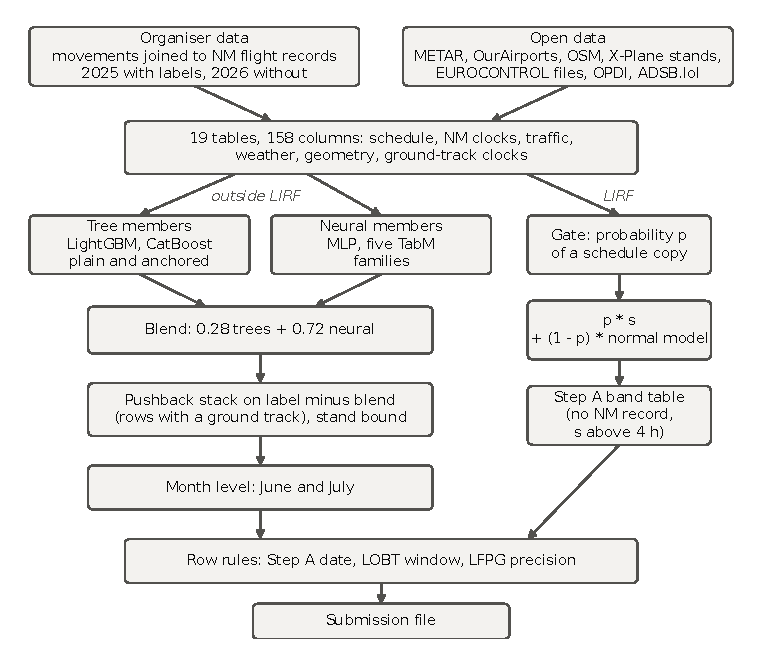
\includegraphics[width=0.75\textwidth]{figures/pipeline.pdf}
  \caption{Stages of the served model. $p$ is the probability of a schedule copy at LIRF; $s$ is the take-off time minus the scheduled time.}
  \label{fig:pipeline}
\end{figure}

\subsection{Validation protocol}

January and July 2025 are the hold-out: 344,336 departures, the months of the ranking set one year earlier. The price of a change is its MSE change on this hold-out. A member fits on the other ten months and stops early on November and December. The served member then fits on all twelve months with the round count of the hold-out fit, scaled by the row ratio.

We set four rules for the season:
\begin{enumerate}
  \item An upload needs a hold-out price of $-150$ MSE or better.
  \item An upload holds one change, so that the live score prices that change.
  \item The team accepts an upload only if its live score is at least 0.3~s below the best. A refit with new seeds moves the live score by about 0.15~s.
  \item No row value comes from a leaderboard score.
\end{enumerate}
Most uploads followed these rules. Some uploads had no hold-out price, and from 8 October 2026, near the deadline, the team judged some uploads on the live score alone. \texttt{RECAP.md} in the repository marks each exception.

\subsection{Columns}

The tree members read 158 columns (Table~\ref{tb:columns}). The operator encoders use the 2025 labels. They are fit on all twelve months both at fit time and at serve time. An out-of-fold version lost 2.3~s on the leaderboard, because the encoder at serve time must match the encoder at fit time.

\begin{table}[htbp!]
  \centering
  \small
  \caption{Column groups of the tree members}
  \label{tb:columns}
  \begin{tabular}{lrp{0.62\textwidth}}
  \toprule
  \textbf{Group} & \textbf{Columns} & \textbf{Content} \\
  \midrule
  Categorical & 10 & Airport, destination, runway, stand, aircraft type, wake class, market segment, operator, flight rule, flight type \\
  Calendar & 3 & Hour, weekday, month \\
  Schedule and plan & 17 & Take-off minus the scheduled, initial and flight-plan off-block times \\
  NM clocks of the flight & 5 & $t_{\mathrm{to}} - \texttt{AOBT\_3}$, $t_{\mathrm{to}} - \texttt{LOBT}$, their gaps to the plan \\
  Later departures & 8 & NM clock of departures in the next 15 and 30~min \\
  Neighbour plan & 18 & Quantiles of the plan delay of departures near in time, queue order \\
  Traffic & 22 & Departures and arrivals in the last 15, 30 and 60~min, per runway \\
  Turnaround & 5 & Ground time and delay of the arrival on the same stand \\
  Operator encoders & 16 & 2025 taxi-out statistics per operator, runway, hour and stand \\
  Weather & 18 & Wind components, visibility, ceiling, temperature, precipitation \\
  Geometry & 9 & Stand and threshold positions, length of the shortest taxi path \\
  OPDI clocks & 4 & Exit-parking and entry-runway events of the flight \\
  ADS-B clocks & 23 & Ground segment, first move, stops, last point at the stand \\
  \bottomrule
  \end{tabular}
\end{table}

The NM clocks of later departures use the departures that take off after the scored flight. They describe the queue in which the flight stood. The organisers allowed columns from other movements and the use of \texttt{AOBT\_3} and \texttt{LOBT}.

\subsection{Ground-track clocks}

The ADS-B clock of a flight needs three steps.
\begin{enumerate}
  \item \textbf{Link.} The builder links a departure to an aircraft by its NM callsign. A departure without an NM record has no callsign, so the builder then tries the flight number. For airports that report IATA flight numbers, it maps the IATA airline code to the ICAO code that the record rows pair with the same number. As a last step, the builder matches the lift-off: the first airborne point within 60~s of a ground point. The lift-off follows the reported take-off time by a fixed offset per airport (for example $-24$~s at EHAM and $+30$~s at LFPG, standard deviation 9 to 22~s). The time and the aircraft type select the callsign aircraft on 99.4\% of the departures that have a callsign.
  \item \textbf{Segment.} The builder walks back from the take-off through the ground points, up to 6~h. A silence above 300~s ends the segment. The receivers often lose an aircraft on the last part of the taxi, so a segment can end up to 3,600~s before the take-off.
  \item \textbf{Clock.} The segment gives the start, the first move, the pushback, the stops and the last point at the assigned stand. The stand positions come from OpenStreetMap. Where OpenStreetMap has no node for the assigned stand, the position comes from the X-Plane Scenery Gateway (five airports).
\end{enumerate}
The OPDI clock uses the exit-parking and the entry-runway events of the flight.

The clocks are not the label. After the removal of a bias, 57\% to 86\% of the linked departures lie within 60~s of the label. A departure that pushes back, waits and moves again can show its first move before the reported off-block: at EHAM, 41\% of the rows do. For this reason the model learns when to trust a clock and does not copy it.

Figure~\ref{fig:coverage} shows the coverage on the ranking set. It is high at EDDM, EHAM, LEBL and LSZH. It is low at LFPG and LIRF and zero at LTFM: we found no open source with ground coverage at Istanbul.

\begin{figure}[htbp!]
  \centering
  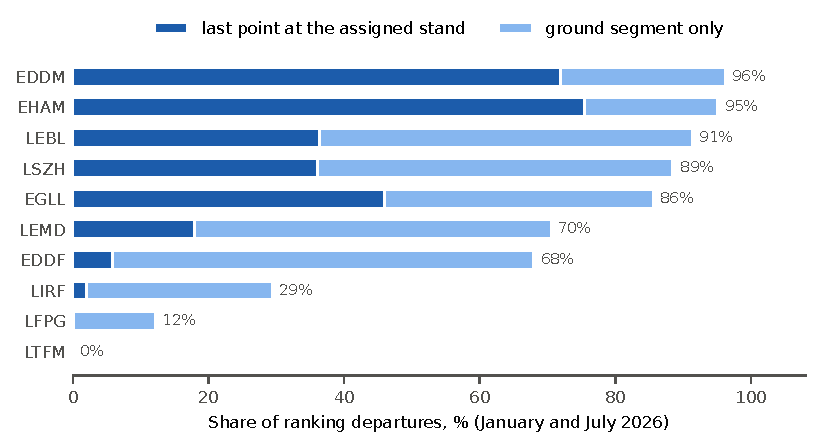
\includegraphics[width=0.9\textwidth]{figures/coverage.pdf}
  \caption{Share of the January and July 2026 ranking departures with an ADS-B clock, per airport, in the tables of 9 October 2026 (v127). The dark part has a last point at the assigned stand. The number gives the share with any ground segment. The links and segments of v130 to v135 later added an ADS-B clock to 15,967 more departures outside LIRF.}
  \label{fig:coverage}
\end{figure}

\subsection{Base members}

All base members fit on the 2025 departures outside LIRF with a label from 0 to 80,000~s (1,923,953 rows). LIRF and the 24-h labels stay out of the fit. This decision gave $-5.99$~s on the leaderboard: the base does not serve these rows, and their labels pulled the trees away from the taxi-out.

\textbf{Tree members.} A global LightGBM \cite{ke2017lightgbm} with linear leaves \cite{shi2019gradient} uses three seeds, 613 leaves, a learning rate of 0.015 and 3,377 rounds. A 24-trial Optuna study \cite{akiba2019optuna} chose the parameters. One LightGBM per airport uses the same parameters. A CatBoost member \cite{prokhorenkova2018catboost} uses depth 8, a learning rate of 0.08 and 7,385 rounds. Its ordered target statistics encode the categorical columns in a different way from LightGBM. Each class also has an \emph{anchored} member, which learns the correction of the NM clock:
\begin{equation}
\label{eq:anchor}
y_{\mathrm{a}} = y - \min\!\left(\max\!\left(t_{\mathrm{to}} - \texttt{AOBT\_3},\, 0\right),\, 7200\right).
\end{equation}
The anchored member and the plain member make different errors. A row without \texttt{AOBT\_3} keeps the plain member. The tree term gives LightGBM and CatBoost equal weights. Inside each library, the plain and the anchored member have equal weights; inside LightGBM, the global and the per-airport member also have equal weights. A grid search and a non-negative least-squares fit of these weights gave no gain on the leaderboard. Two guards replace a member that differs from the others by more than 3,600~s. A bound per airport caps a value above the 2025 range of the airport.

\textbf{Neural members.} Trees share their errors, and a neural network learns a smoother function of the same columns \cite{grinsztajn2022tree}. A multilayer perceptron uses three hidden layers (1,024, 512 and 256 units), one embedding per categorical column and three seeds. Five TabM families \cite{gorishniy2025tabm}, three seeds each, use 16 sub-models with shared weights. The families differ in the numeric embedding (piecewise linear or periodic \cite{gorishniy2022embeddings}) and in the column set. The neural term and the blend are
\begin{align}
\hat{y}_{\mathrm{nn}} &= 0.35\, \hat{y}_{\mathrm{mlp}} + 0.65\, \bar{y}_{\mathrm{tabm}}, \label{eq:nn}\\
\hat{y}_{\mathrm{b}} &= 0.28\, \hat{y}_{\mathrm{trees}} + 0.72\, \hat{y}_{\mathrm{nn}}. \label{eq:blend}
\end{align}
The neural weight grew from 0.15 to 0.72 over the season.

\subsection{Regime head at Rome Fiumicino}
\label{sec:lirf}

At LIRF, part of the departures report the scheduled time as the off-block time, so $y = s$. In 2025, about 21\% of the LIRF departures of the fit months are fallback rows. The head has four parts.
\begin{enumerate}
  \item \textbf{Gate.} A LightGBM classifier gives the probability $p$ that a row is a fallback row. An isotonic map \cite{zadrozny2002transforming} calibrates $p$ on out-of-fold scores. Each of the six folds holds out one winter month and one summer month. The strongest columns describe the arrivals. An airline that reports its arrivals on the schedule also reports its departures on the schedule (correlation 0.77 over the airline months of 2025). The ranking file keeps the arrival block times, so the 2026 shares exist without a 2026 departure label.
  \item \textbf{Normal model.} Five LightGBM seeds fit on the LIRF rows that are not fallback rows.
  \item \textbf{Value.} The value minimises the expected squared error over the two regimes:
  \begin{equation}
  \label{eq:lirf}
  \hat{y} = p\, s + (1 - p)\, \hat{y}_{\mathrm{norm}}.
  \end{equation}
  \item \textbf{Band table.} A row without an NM record and with $s$ above 14,400~s takes its value from a table of 11 bands of $s$. Each band holds the 2025 shares of the fallback, the normal and the 24-h labels.
\end{enumerate}

\subsection{Pushback stack}

The stacked model \cite{wolpert1992stacked} uses the ground track of the scored flight. It is a LightGBM with 15 leaves, 400 rounds, a learning rate of 0.03, at least 100 rows per leaf and an L2 penalty of 50. Its target is the residual of the blend, clipped to $\pm 3{,}600$~s, and the final value is
\begin{equation}
\label{eq:stack}
\hat{y} = \max\!\left(\hat{y}_{\mathrm{b}} + f(\mathbf{x}),\, 0\right).
\end{equation}
The stack serves the departures outside LIRF that have an OPDI or an ADS-B clock: 216,792 of the 344,841 ranking departures. Its columns are the airport, each clock as its difference to the blend and the quality of the track (points, largest gap, distance of the first point to the stand). Two member gaps complete them: the neural term minus the tree term, and the TabM mean minus the perceptron.

The stack learns on the January and July 2025 hold-out, where the blend is out of sample. A stack that learns on rows that the members fitted on learns a residual that does not exist at serve time. The hold-out has a different coverage mix from 2026: EGLL had a stand clock on 4\% of its departures in 2025 and on 46\% in 2026. Each training row therefore has the weight
\begin{equation}
\label{eq:weight}
w = \min\!\left(\max\!\left(\frac{\pi_{2026}(a, c)}{\pi_{2025}(a, c)},\, 0.2\right),\, 5\right),
\end{equation}
where $\pi(a, c)$ is the share of the coverage class $c$ at the airport $a$. The weights read no label.

A stand bound follows the stack. The taxi-out is at least the time from the last ADS-B point at the assigned stand to the take-off. The bound lifts 930 ranking departures.

\subsection{Month level}

EUROCONTROL publishes the mean taxi-out per airport and month \cite{eurocontrolperf}. This file is an aggregate of the labels of the scored months, so we keep it as a separate step that a flag switches off. The organisers confirmed its use for the scored months. The step moves the values $\hat{y} \le 7{,}200$~s of an airport and month by one shift:
\begin{equation}
\label{eq:month}
\Delta = m_{\mathrm{pub}} + g_{a} - \bar{\hat{y}},
\end{equation}
where $m_{\mathrm{pub}}$ is the published mean, $\bar{\hat{y}}$ is the mean of the served values and $g_{a}$ is the 2025 gap between the label mean and the published mean at the airport $a$. At LFPG the gap is a line on the share of departures that the file drops. A month moves only if three conditions hold. The month lies in April to October. The leave-one-month-out error of the gap is at most 8~s. The kept share lies in the 2025 range of the airport. In winter the file drops the long departures and the gap grows to 164~s. LIRF does not move. The step moves 7 airport months of the ranking set and 14 of the final set, by $-33$~s to $+32$~s.

\subsection{Row rules}

Three rules set single rows. Each follows from a fact of the 2025 data, not from a score.
\begin{enumerate}
  \item \textbf{Date fix.} The band table holds a share of 24-h labels. A 24-h label needs a change of the local date between the schedule and the take-off. Where the two dates are equal, the rule removes the 24-h term. The rule moves 1 ranking row.
  \item \textbf{Join window.} The organisers joined a movement to its NM flight only if the off-block time lies within 3,606~s of \texttt{LOBT}. Each 2025 row with a record obeys this. So the label lies within 3,606~s of $t_{\mathrm{to}} - \texttt{LOBT}$, and the rule projects each prediction into this window. The same window sets $p = 0$ at LIRF where a schedule copy would break it. The rule moves 59 ranking rows.
  \item \textbf{Precision at LFPG.} At LFPG each take-off time is a whole minute plus the organiser noise. A take-off time off this grid marks an off-block near \texttt{LOBT}. In 2025 the median label of these rows is 4,453~s, against 1,191~s on the grid. The rule raises these rows to $t_{\mathrm{to}} - \texttt{LOBT} - 242$~s, the 2025 median offset, and never lowers a row. It moves 18 ranking rows.
\end{enumerate}


\section{Results}
\label{sec:results}

\subsection{Leaderboard path}

Figure~\ref{fig:path} shows the live RMSE of the 106 scored uploads. Table~\ref{tb:path} in the appendix lists the uploads that added a new mechanism. The final recipe, v139, scores 231.90~s. On 13 October 2026, at the end of the ranking phase, this was rank 21 of 246 teams; the best team scored 212.85~s.
% TODO(authors): add the final-phase RMSE and rank after the organisers publish them (OpenSky Symposium, 29-30 October 2026).

\begin{figure}[htbp!]
  \centering
  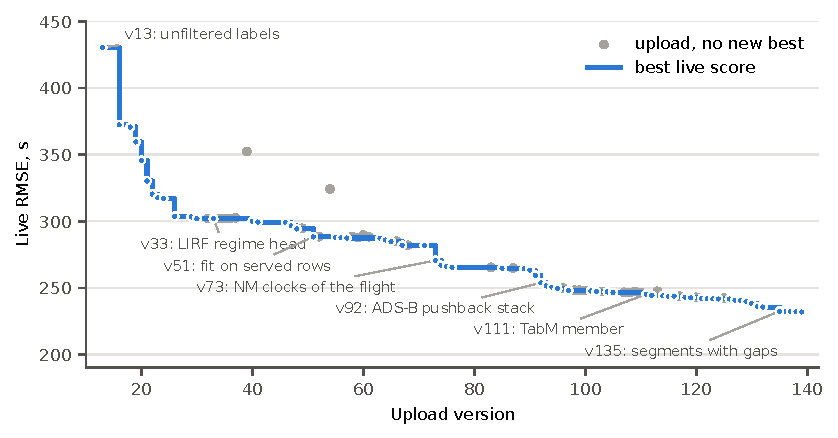
\includegraphics[width=\textwidth]{figures/score_path.pdf}
  \caption{Live RMSE of each scored upload on the January and July 2026 ranking set. Uploads v1 to v10 scored 560.91~s to 562.44~s with filtered labels and are not shown.}
  \label{fig:path}
\end{figure}


The path has three phases. Up to v51, the gains came from the label. The first models filtered the labels to 30 to 7,200~s and clipped the predictions, so they could not learn the long labels. The removal of the filter and the clip, together with the plan columns, gave 130~s. The LIRF head and the decision to fit the base on the served rows followed. From v73 to v135, the gains came from new measurements of the off-block. The NM clocks gave $-11.3$~s, and the OPDI and ADS-B clocks gave $-15.5$~s in six uploads. The links that raised the coverage of the ground tracks gave $-9.2$~s from v127 to v135. The neural members added about 4~s between v94 and v126.

\subsection{Error budget}

Table~\ref{tb:budget} splits the error of v135 by coverage class. The hold-out RMSE of each class is projected onto the 2026 mix of the classes.

\begin{table}[htbp!]
  \centering
  \small
  \caption{Error budget of v135 outside LIRF, labels up to 7,200~s. Hold-out: January and July 2025. Projected MSE: the hold-out error per row on the 2026 mix, ranking scale.}
  \label{tb:budget}
  \begin{tabular}{lrrrr}
  \toprule
  \textbf{Coverage class} & \textbf{Hold-out rows} & \textbf{RMSE, s} & \textbf{2026 rows} & \textbf{Projected MSE} \\
  \midrule
  Last point at the assigned stand & 64,698 & 93.4 & 96,221 & 2,854 \\
  ADS-B segment to the take-off & 85,565 & 164.9 & 104,808 & 8,699 \\
  ADS-B segment that ends earlier & 18,637 & 169.8 & 13,948 & 1,102 \\
  OPDI only & 988 & 176.8 & 1,815 & 75 \\
  No clock & 147,865 & 217.0 & 101,150 & 15,251 \\
  \midrule
  Sum & & & 317,942 & 27,981 \\
  \bottomrule
  \end{tabular}
\end{table}

The live MSE of v135 is 54,034. The classes of Table~\ref{tb:budget} hold about 27,981 of it. LIRF and the labels above 7,200~s at the other airports hold the rest, about 26,050 (48\%). On the hold-out, 36 rows above 7,200~s hold 32,073 of 62,347 MSE outside LIRF. The rows without a clock hold most of the remaining normal error: 7,406 at LTFM and 5,149 at LFPG.

\subsection{Hold-out price against live change}

Table~\ref{tb:transfer} compares the hold-out price of nine uploads with their live change. The live change is the difference of the squared live RMSE. The two scales have almost the same row count (344,336 against 344,841).

\begin{table}[htbp!]
  \centering
  \small
  \caption{Hold-out price and live change, both in MSE. A negative value is a gain. The v73 price is the price of one member against a control with equal rounds.}
  \label{tb:transfer}
  \begin{tabular}{llrr}
  \toprule
  \textbf{Upload} & \textbf{Change} & \textbf{Hold-out price} & \textbf{Live change} \\
  \midrule
  v32 & Seven seeds in the base mean & $-1{,}204$ & $+79$ \\
  v37 & Five seeds in the LIRF gate & $-151$ & $+393$ \\
  v46 & Three base changes with a new parameter study & $-1{,}864$ & $-102$ \\
  v96 & ADS-B specialist model as a stack column & $-302$ & $+265$ \\
  v73 & NM clocks of the flight & $-5{,}652$ & $-6{,}237$ \\
  v97 & ADS-B columns in each base member & $-983$ & $-746$ \\
  v135 & Segments that end before the take-off & $-1{,}660$ & $-1{,}445$ \\
  v111 & TabM member & $-231$ & $-615$ \\
  v137 & Two member gaps as stack columns & $-76$ & $-116$ \\
  \bottomrule
  \end{tabular}
\end{table}

Two patterns appear. Seed averages, parameter studies and derived columns gained on the hold-out and lost on the leaderboard. New row-level measurements transferred at 0.76 to 1.10 of their price. Neural members gained 1.5 to 2.7 times their price.

\subsection{Changes that failed}

The repository records each failed change with its price and its live score. The most instructive are:
\begin{itemize}
  \item \textbf{A base that learns only the residual from an anchor} (the plan or the schedule) lost 35.9~s. On a delayed flight the anchor is wrong by hours. The anchored members of Equation~\ref{eq:anchor} work because the NM clock is a measurement and the plain member stays in the blend.
  \item \textbf{Rules for long labels outside LIRF} cost 1,639 MSE on the hold-out. Outside LIRF, 412 rows of 2025 have no NM record and an $s$ above 14,400~s. None of them lies within 60~s of $s$, so the LIRF regime does not exist there.
  \item \textbf{A lower bound from the first ADS-B ground point} cost 4,875 to 7,954 MSE on the hold-out. The first point often moves before the reported off-block.
  \item \textbf{Every later change of the LIRF head} lost on the leaderboard: a CatBoost gate ($+0.89$~s), a TabM gate ($+3.12$~s) and a gate with the NM clocks ($+0.67$~s).
  \item \textbf{Huber and log-target losses} scored a hold-out RMSE of 408~s. The metric is the RMSE, so the loss must be the squared error.
\end{itemize}

\subsection{Final phase}

On 8 October 2026 the organisers added February and June 2026 to the scored months, to limit fits to the leaderboard. The final file holds 670,790 departures. It uses the v139 recipe and the saved fits, so no model learns on the final months. On the 344,841 shared departures it differs from v139 by 6.7~s on average, because the organisers drew a new timestamp noise. One known gap affects February: EDDF has no ground coverage from 2026-01-29 to 2026-02-28 in ADSB.lol and OPDI, so 10,367 February departures have no clock. We estimate the cost near 230 MSE on the final scale.


\section{Discussion}
\label{sec:discussion}

\subsection{A post-operational estimator}

The model reads the take-off time, the NM records and the ground track up to the take-off. It cannot run before the off-block, so it does not support departure management. It suits the post-operational use that motivates the challenge. It fills a missing off-block time and checks a reported one. It also gives the taxi-out time of a past flight where the airport report is not open. For this use, the clocks from open ADS-B traces are the main result. They are physical observations of the off-block, and each new link that attached a track to more departures paid on the leaderboard.

\subsection{Parts that model the data set}

Four parts of the model follow how the labels were made, not how the aircraft taxied: the LIRF head, the band table, the join-window rule and the LFPG precision rule. The LIRF head models a real reporting practice of an airport, and it is a data-quality finding in its own right. The join-window rule follows from how the organisers built the data set, and the precision rule follows from how they added noise. These two rules move 77 ranking rows. On the hold-out, the join window prices $-371$ MSE, the same window at the LIRF gate $-193$ MSE and the precision rule $-250$ MSE. The join window alone gave $-0.85$~s on the leaderboard (v118); the other two went up in uploads with a second change. The rules do not transfer to another data set. A user who wants an estimate of the physical taxi-out time must remove all four parts. We publish them for two reasons. The challenge rewards the exact label, and the same facts help the data owners to find the rows with a doubtful off-block time.

The month level reads an aggregate of the labels of the scored months. It gave 0.30~s (v138 and v139). The model without it is v137, with 232.20~s. We report both.

\subsection{Reuse of the leaderboard}

The team scored 106 uploads against one ranking set. Each use of a fixed test set adapts the model to it and biases the score down \cite{blum2015ladder,dwork2015reusable}. Three controls limited this effect. Every change had a hold-out price before the upload. The acceptance bar of 0.3~s was twice the noise of a refit. No row value came from a score. Near the deadline the team accepted three uploads below the bar (v137 to v139); it wrote the acceptance rule of each before the upload. Table~\ref{tb:transfer} shows that the hold-out and the leaderboard disagreed often enough to make the leaderboard a second validation set in practice. The final phase added two unseen months for this reason. Its score is the fair test of the recipe.

\subsection{Limits}

\begin{itemize}
  \item \textbf{Coverage.} LTFM has no open ground track, and LFPG had a ground segment on 12\% of its departures in the tables of Figure~\ref{fig:coverage}. These two airports hold most of the error of the rows without a clock.
  \item \textbf{Long labels.} A label above 7,200~s outside LIRF is not predictable from the columns. The final file holds 160 values above 7,200~s.
  \item \textbf{Stack data.} The stack learns on two months of 2025, the months where the blend is out of sample.
  \item \textbf{Cost.} The served recipe holds 80 trained artefacts (14~GB). A full refit takes about 20~h on a 16-thread processor and about 10~h on a graphics processor for the TabM families. A smaller model would be easier to maintain; we did not measure the score of a distilled model.
\end{itemize}

More ground receivers near Paris, Rome and Istanbul would reduce the error more than any change of the learner. On the hold-out, a departure with a stand clock has an RMSE of 93~s, and a departure without a clock has 217~s.


\section{Conclusion}

The taxi-out label of the challenge is a report with airport-specific regimes, and the best predictor of it is an independent measurement of the off-block. Open ADS-B traces and OPDI events give such a measurement for 68\% of the scored departures outside Rome Fiumicino. With a blend of trees and TabM networks, a stacked model on the clocks and a regime head at Rome Fiumicino, the model scores 231.90~s RMSE on the ranking set. The upload log shows that new measurements transferred from the hold-out to the leaderboard, and that tuning did not. The ground coverage of open ADS-B networks now limits the error more than the model.


\appendix

\section{Uploads with a new mechanism}

\begin{table}[h!]
  \centering
  \small
  \caption{Uploads that added a new mechanism. RMSE on the 344,841 ranking departures.}
  \label{tb:path}
  \begin{tabular}{lrl}
  \toprule
  \textbf{Upload} & \textbf{RMSE, s} & \textbf{Mechanism} \\
  \midrule
  v13 & 430.45 & Unfiltered labels; schedule and plan terms \\
  v21 & 330.12 & LightGBM with linear leaves; first LIRF rules \\
  v33 & 301.87 & LIRF regime head: gate, normal model, band table \\
  v47 & 296.57 & Fit on the 12 months of 2025 \\
  v51 & 288.25 & Base fit on the served rows only \\
  v67 & 281.87 & CatBoost as a second tree library \\
  v73 & 270.58 & NM clocks of the scored flight \\
  v74 & 266.84 & Anchored LightGBM member; NM clocks in CatBoost \\
  v76 & 265.27 & New parameter study \\
  v89 & 264.34 & Clocks of later departures; LightGBM per airport \\
  v92 & 253.82 & OPDI and ADS-B clocks in a stack; stand bound \\
  v97 & 247.89 & ADS-B columns in each base member \\
  v105 & 246.48 & Airline arrival columns in the LIRF gate; perceptron \\
  v111 & 245.23 & TabM member \\
  v115 & 243.69 & X-Plane stand positions \\
  v118 & 242.81 & Join window of the NM record \\
  v121 & 242.03 & LFPG precision rule \\
  v127 & 240.70 & Ground tracks for departures without an NM record \\
  v130 & 238.25 & Lift-off link \\
  v131 & 235.95 & TabM families refit on the new tables \\
  v135 & 232.45 & Segments that end before the take-off \\
  v137 & 232.20 & Two member gaps as stack columns \\
  v139 & 231.90 & Month level \\
  \bottomrule
  \end{tabular}
\end{table}


\section*{Acknowledgement}
We thank the EUROCONTROL Performance Review Commission and the OpenSky Network for the challenge data and its organisation. We thank the contributors of ADSB.lol, OpenStreetMap, OurAirports, the Iowa Environmental Mesonet, the OPDI project, the X-Plane Scenery Gateway and the Virtual Radar Server community for their open data. The use of $t_{\mathrm{to}} - \texttt{AOBT\_3}$ as a clock is public in the repositories of other teams of the challenge; our code copies none of them.

\section*{Use of generative AI}
% TODO(authors): confirm that this statement is complete and true before submission.
The authors used an AI coding assistant (Claude Code, Anthropic) to write and audit parts of the code and to draft this manuscript. The authors checked the content and take full responsibility for it.

\section*{Author contributions}
% TODO(authors): assign the CRediT roles.
\begin{itemize}
  \item First Author: Conceptualization, Methodology, Software, Validation, Writing (Original Draft).
  \item Second Author: Data Curation, Software, Investigation, Writing (Review and Editing).
\end{itemize}

\section*{Funding statement}
% TODO(authors): confirm.
This research received no external funding.

\section*{Open data statement}
The challenge data belong to the EUROCONTROL Performance Review Commission and the OpenSky Network. Registered teams received them during the challenge. The organisers plan to publish them as open data together with a data paper in JOAS.
% TODO(authors): cite the DOI of the challenge data set when it is published.
Each other source of Table~\ref{tb:sources} is open, and the command \texttt{python -m src\_v3.fetch\_external} of the repository downloads it. The tables derived from ADSB.lol stay out of the repository because of the share-alike clause of the ODbL; the same command rebuilds them. The data of the figures are in \texttt{paper/data} of the repository.

\section*{Reproducibility statement}
The source code is public under the GNU GPLv3 \cite{kindmango2026repo}.
% TODO(authors): add the tag or the commit of the paper version, and a Zenodo DOI of the repository if you archive it.
\texttt{REPRODUCE.md} gives the commands that rebuild the final file: \texttt{python -m src\_v3.release\_final tables}, then \texttt{serve} with the flags of v139. A second run of \texttt{serve} rebuilt the final file of v135 with the same SHA-256. \texttt{python -m src\_v3.test\_parity --version 92} rebuilds the file of v92 bit for bit from the saved fits. \texttt{RECAP.md} records the price and the live score of each upload. The script \texttt{paper/make\_figures.py} draws each figure of this paper from the data in \texttt{paper/data}. The repository does not host the 80 trained artefacts (14~GB); \texttt{REPRODUCE.md} gives the fit command of each.

\printbibliography

\end{document}
